\documentclass[a4j,11pt]{jsarticle}
\usepackage{semi}
 \usepackage{url}
\makeatletter % プリアンブルで定義開始

% 図番号を"<章節などの番号番号> - <図番号>" へ
\renewcommand{\thefigure}{\thesubsection-\arabic{figure}}
\renewcommand{\thetable}{\thesubsection-\arabic{table}}
% 章が進むごとに図番号をリセットする
\@addtoreset{figure}{subsection}
\@addtoreset{table}{section}
\renewcommand{\theequation}{% 式番号の付け方
	\thesection.\arabic{equation}}
	\@addtoreset{equation}{section}
\makeatother % プリアンブルで定義終了

\renewcommand{\headfont}{\bfseries} %章タイトルなどを明朝体にする

\makeindex
\begin{document}
\definecolor{cellcolor}{rgb}{ 1, .90, .90}
\definecolor{rowcolor}{rgb}{.85, .85, 1}
\setcounter{tocdepth}{3}
\thispagestyle{empty}
\clearpage
\addtocounter{page}{-1}
\begin{center}

\huge
2020年度 卒業論文\\[60pt]
\HUGE
逆畳込みとケプストラム法を\\
組み合わせることによる\\
残響除去の提案\\[65pt]
\huge
指導教員 須田 宇宙 准教授\\[40pt]
千葉工業大学 情報ネットワーク学科\\[10pt]
須田研究室\\[40pt]
1632038 \hspace{70pt} 岡田 秀\\[110pt]
\end{center}
\begin{flushright} 
\huge

\textcolor{white}{文字}

\textcolor{white}{文字}

提出日 2020年1月24日
\end{flushright}
\newpage
\thispagestyle{empty}
\clearpage
\addtocounter{page}{-1}
\large
% 目次
\tableofcontents
\thispagestyle{empty}
\clearpage
\addtocounter{page}{-1}
\newpage
%表目次
\listoftables
%図目次
\listoffigures
\thispagestyle{empty}
\clearpage
\addtocounter{page}{-1}
\begin{comment}

\end{comment}
\newpage

\section{緒言}

%背景+問題点
近年,災害が多発している中,町内放送などの非常放送が重要性を増している\cite{oka1}.屋外,デパートなどの屋内,トンネルの中など様々な場所で館内放送や非常放送の整備されている.しかし,スピーカから離れている地点で放送を聞くと建物などによる反射音により,内容を聞き取りづらいことが多い.ここで,信号処理によって反射音を除去できれば,放送内容を聞き取ることが可能となる.

火災が発生した場合,屋内のスピーカからの非常放送を屋内で受聴することになるが,反射や残響によって聞き取りづらいことが懸念される.
一方,建築音響の分野では,単発の信号音に対する反射音の時間遅れとその大きさを表す指標としてインパルス応答が用いられる.反射音を除去する方法として佐藤\cite{oka2}の研究では非常用放送の音声の先頭に信号音を付加させた.その信号音を基準とし,デジタルデバイスによってリアルタイムにインパルス応答を計算し,余分な反射音を除去する手法を提案した.しかし,クロススペクトル法の理論は正しかったが,実際の音声を用いて計算したところうまく動作しなかった.


%目的
本研究では,佐藤\cite{oka2}の研究の理論の部分を逆畳込みとケプストラム法を用いて非常放送を明瞭に聞き取ることを目的とする.

\subsection{行政放送などの公共放送における問題点}
行政放送や,公共放送などは津波や地震,火災といった人の命に関する放送することが多くある.そのような重要な放送は時と場所によっては内容が聞き取りづらい,または聞き取れない,ことがある.

一つ例を挙げるとすると2011年3月11日に発生した東日本大震災がある.被災地において,普段は行政無線などの広域拡散情報通信システムは,隣接するスピーカーからの音が重ならないよう,十分な時間間隔を開けて出力している.しかし,当時は津波の避難を迅速に行わなければいけないこと,自分自身も避難しなければいけないことなどがあり,十分な時間間隔を開けることができなく放送を行ってしまった.結果としてスピーカ同士の干渉であったり,建物などによる反射により内容を十分に聞き取ることができなかったという問題が発生した.


\newpage

\section{行政放送}
行政放送は市町村防災行政無線のことをいい,主に地方行政における無線の一種である.放送内容は大規模災害時の避難勧告や避難命令などの告知,火災発生の知らせといった非常時の放送を始め,朝・昼・夕方の時報を知らせる音楽.鐘・サイレン・チャイムや児童に帰宅を促す放送などがある.放送のほとんどは遠方にある野外スピーカからの声が重なって聞き取りにくくなるのを防ぐため,語間を大きく開け,ゆっくり話す,または,放送区域を時間差で切り替える時間差放送を行っているのが特徴である.



\newpage

\section{津波や地震や火事による自然災害}
津波は主に地震や火山活動による海底の地形の急変により,海洋に生じる大規模な波のことであり,自身による津波は海溝付近で発生することが多い.2011年に発生した東日本大震災の津波は観測史上最大級規模のの津波であり,震源地は仙台市の東方70km出会ったが,北海道から千葉県にかけて大津波が押し寄せている.

津波の伝搬する速度は水深と波の高さによって決まり,基本的には重力加速度に水深を乗じた値の平方根に等しくなっている.東日本大震災では震源地から岩手県重茂半島まで平均時速115kmで到達しており,津波の高さは同書で8.5mとなっている.しかい,津波が強すぎたためか観測データが送信されておらず,実際にはもっと高かった可能性もある.宮城県女川町では鉄筋コンクリート製のビルが基礎の部分から自演から抜けて横倒しになってしまっている.

津波の強さは,高さ1mでの破壊力があり,成人男性であっても死亡してしまう可能性がある.また,木造建築であれば全壊してしまう可能性がある.また,津波は陸から海へ引く,引波の際の力も強く,時折,湖岸で釣りをしていた釣り人が沖合に流されてしまうニュースもある.

地震が起きた際の津波の発生原理を示す.海底で地震が発生すると海底の地盤が動き,海側のプレートと陸側のプレートの隆起と沈降が起こる.プレートの隆起と沈降に合わせて上げ潮や引き潮が発生し,津波につながる.津波はお気から騎士につかづくほど波が高くなり,水深が深ければ深いほど速度が早くなる.

\newpage
 % 図3.0-1
\begin{figure}[h]
\begin{center}
 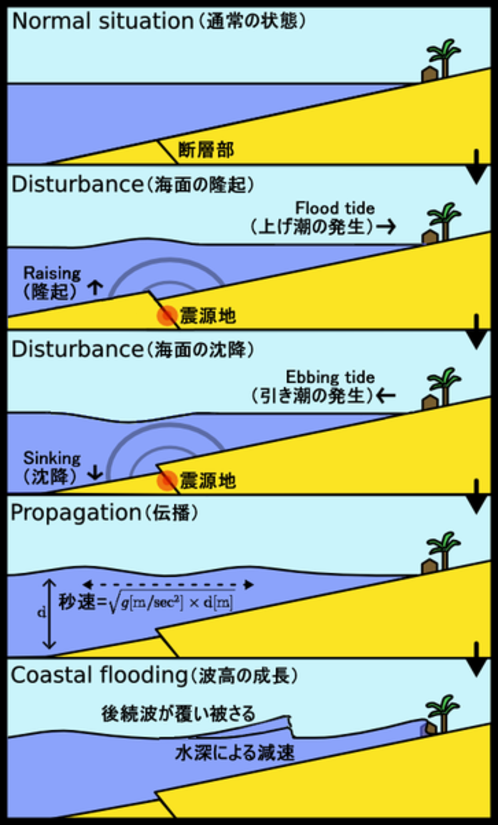
\includegraphics[clip,width=100mm,height=100mm]{eathquack.pdf}
\end{center}
 \caption{津波の発生原理\cite{oka2}}
 \label{fig:eathquack}
\end{figure}

図\ref{fig:eathquack}に地震が起きた際の津波の発生原理を示す.海底で地震が発生すると海底の地盤が動き,海側のプレートと陸側のプレートの隆起と沈降が起こる.プレートの隆起と沈降に合わせて上げ潮や引き潮が発生し,津波につながる.津波は沖から岸に近づくほど波が高くなり,水深が深ければ深いほど速度が早い.

\newpage


\section{信号処理}
信号処理とは,信号(光・音声・画像信号など)を数理手法で処理(分析・加工)する学問・技術の総称である.

アナログ信号処理とデジタル信号処理に分けられる.信号処理を支える基礎的な分野は信号理論とも呼ばれる.

基本的には,信号から信号に変換するものであり,信号とは別の形式の情報を得るもの(例えば、カテゴリ分けや関連づけ,推論的な情報を得る認識や理解など)は含まれない.圧縮も含まれないことが多い.但し,認識や理解,圧縮の前段階としての信号の変換は信号処理と呼ばれる.そのため,信号処理はそれらの技術に対して非常に重要であるとともに関連が強い.なお,また入力と出力が同じ種類(物理量)の信号である場合(例えば入力と出力ともに同じ音圧である場合)には,フィルタリングとも呼ばれる.

信号処理の例としては,ノイズの載った信号から元の信号を推定するノイズ除去や,時間的な先の値を推定する予測,時間周波数解析などを行う直交変換,信号の特徴を得る特徴抽出,特定の周波数成分のみを得るフィルタなどがある.

高速フーリエ変換,ウェーブレット変換,畳み込み等のアルゴリズムがあり,以前はそれぞれ専用のハードウェアで処理していたが,近年ではDSPや汎用のハードウェアでソフトウェアで処理したり,FPGAによる再構成可能コンピューティングによって処理する方法が開発されつつある.


\subsection{周波数}
周波数とは,高額,特に電気工学・電波工学や音響工学などにおいて,電気振動(電磁波や振動電流)などの現象が,単位時間(Hzの場合は1秒)あたりに繰り返さる回数のことである.
\subsubsection{周波数特性.周波数領域}
周波数特性とは,周波数と何らかの物理量との関係を表したものである.直流電流ならば単純に比率(ゲイン)だけで伝達特性を定義できる.しかし,実際の被測定物では,周波数によって伝達特性が変化する.さらに交流では比率(ゲイン)だけでなく,入出力間の位相差も問題となる場合が多い.
\subsubsection{フーリエ級数展開}
すべての周期信号は基本周波数の正弦波,余弦波人,その整数倍の周波数を持つ正弦波,余弦波の重ね合わせとして表現できる.このことから周期信号による音を純音に対して複合音という.
すべての周期信号は式(\ref{furie})のように表すことができる.

\begin{equation}
	\label{furie}
  y(t) = a_{0} + \sum^{\infty}_{K=1} (a_{k}cos k\omega_{0}t +  b_{k}sin k\omega_{0}t) 
\end{equation}

ここで$a_{0}$は直流成分,$a_{k}$,$b_{k}$はそれぞれ正弦波,余弦波の係数である.周期信号をこのような正余弦波の成分に展開することをフーリエ級数展開という.
また,$a_{k}$,$b_{k}$をフーリエ係数という.

\subsubsection{フーリエ変換}
フーリエ級数展開では,時間的に連続な信号を基本周波数とその倍数の成分の大きさの数字列で表したことになる.このような解析はコンピュータで行うことが主流なので,解析の対象となる信号も連続信号ではなく,時系列と呼ばれる離散的なデータである.また,実際の音の信号を解析する場合は信号の周期を正確に取り出し,解析することは容易ではない.

そこで,実用的な方法として,音の信号を時系列として取り込み,その中から解析したい部分のデータを取り出す.そして,その切り出したデータの長さ分を周期としてみなし,その周期のなす基本周波数とその倍数の成分の係数としてスペクトルを求める.

しかし,このような周期信号は一般的に不連続につながるので,不連続部分が高い周波数の成分として扱われてしまう.そこで窓掛けと呼ばれる処理によって波形の接続部分をなめらかに変形してから解析する.

このように時系列データを周波数のデータ,すなわちスペクトルに変換する方法を離散フーリエ変換(DFT:Discrete Fourier Transform)
という.また,またその逆を離散フーリエ逆変換(IDFT)という.離散フーリエ変換には計算を高速化する手法が開発され,周期とみなすデータ数を2のべき乗に選んだ場合には高速フーリエ変換(FFT:Fast fourier Transform)と呼ばれる方法が使われる\cite{oka3}.

\newpage
\section{室内音響}
\subsection{残響音・反響}
室内などの閉空間内で発生した音は壁にあたって反射する.反射した音は別の壁による反射を繰り返し,次第に減少していく.このような多重の反射が作り出す現象を残響という.直接音から反射がなくなるまで減衰の包括線は続いていく.
残響により,音声が重複してしまったり,エコーが掛かって聞こえなくなってしまうことがある.
その様子を波形にしたものを図\ref{fig:hakei}に示す.

% 図5.1-1
\begin{figure}[h]
\begin{center}
 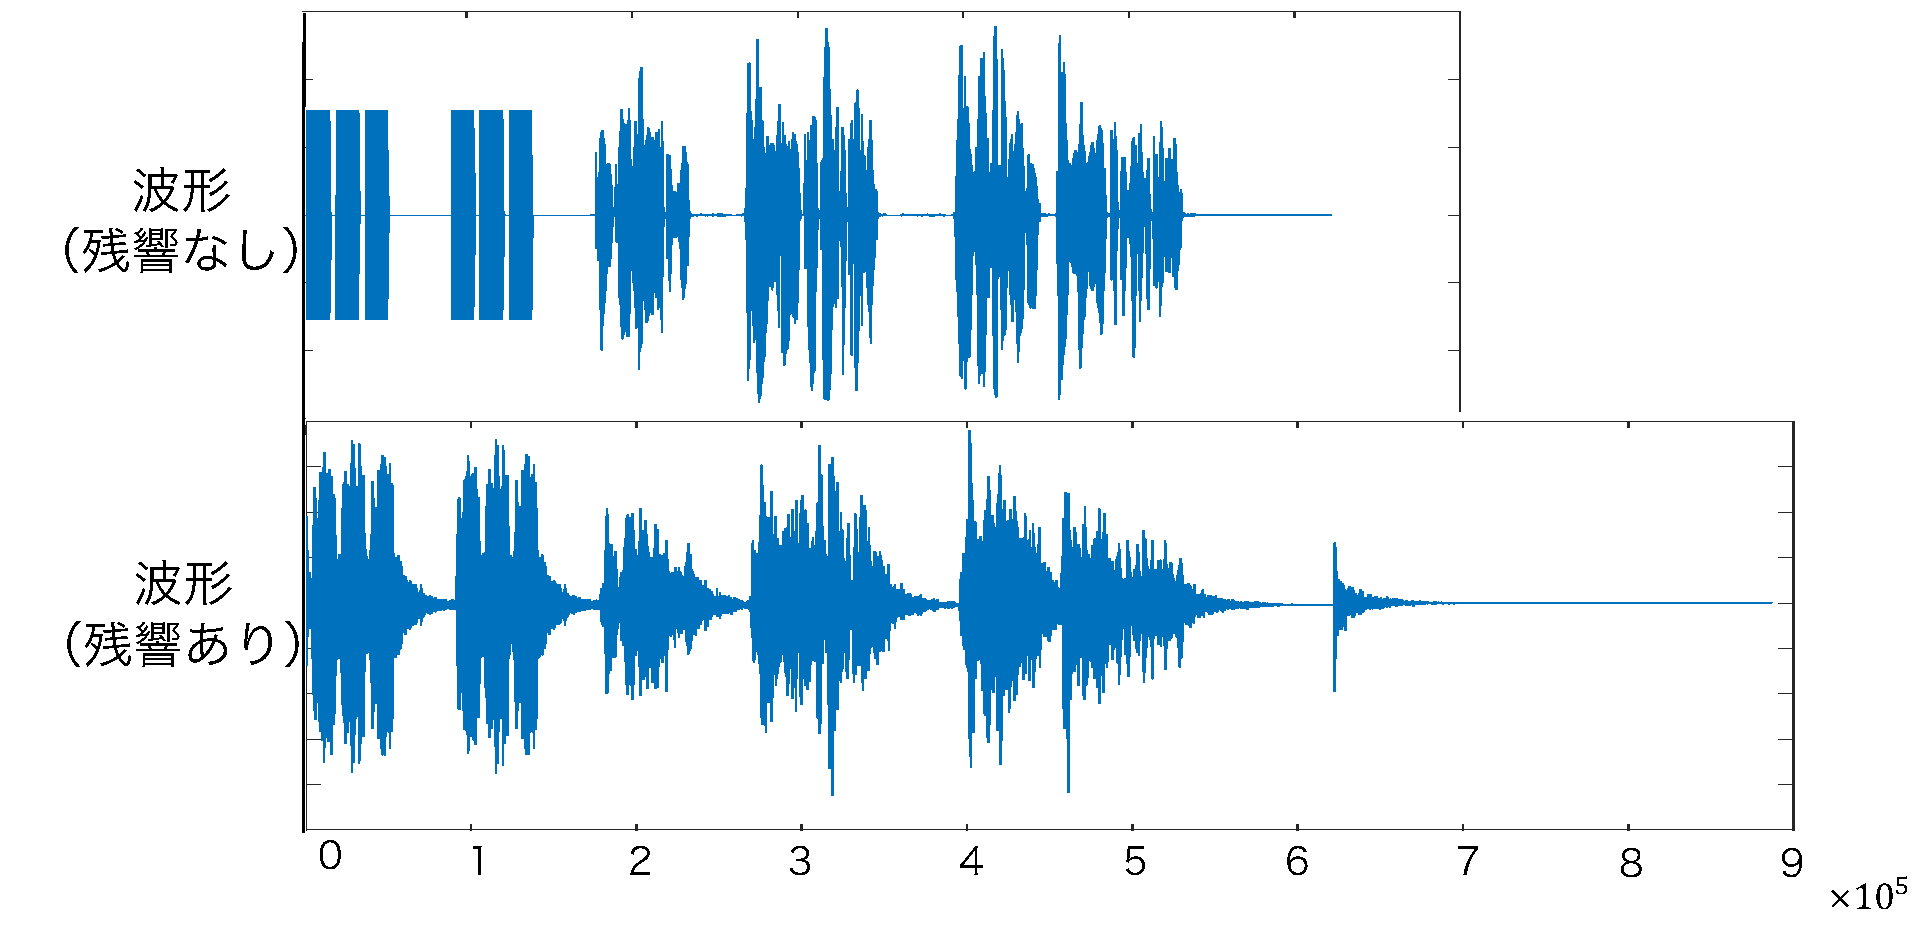
\includegraphics[clip,width=130mm,height=80mm]{hakeikekka.pdf}
\end{center}
 \caption{残響影響波形例}
 \label{fig:hakei}
\end{figure}

\subsection{インパルス応答}
音源から単一の衝撃音を発したときの受音点での音の観測結果は例を図\ref{fig:impulse}に示す.直接音をインパルスと呼び,それに対する空間情報すべてをインパルス応答と呼ぶ\cite{oka3}.

% 図5.2-1
\begin{figure}[h]
\begin{center}
 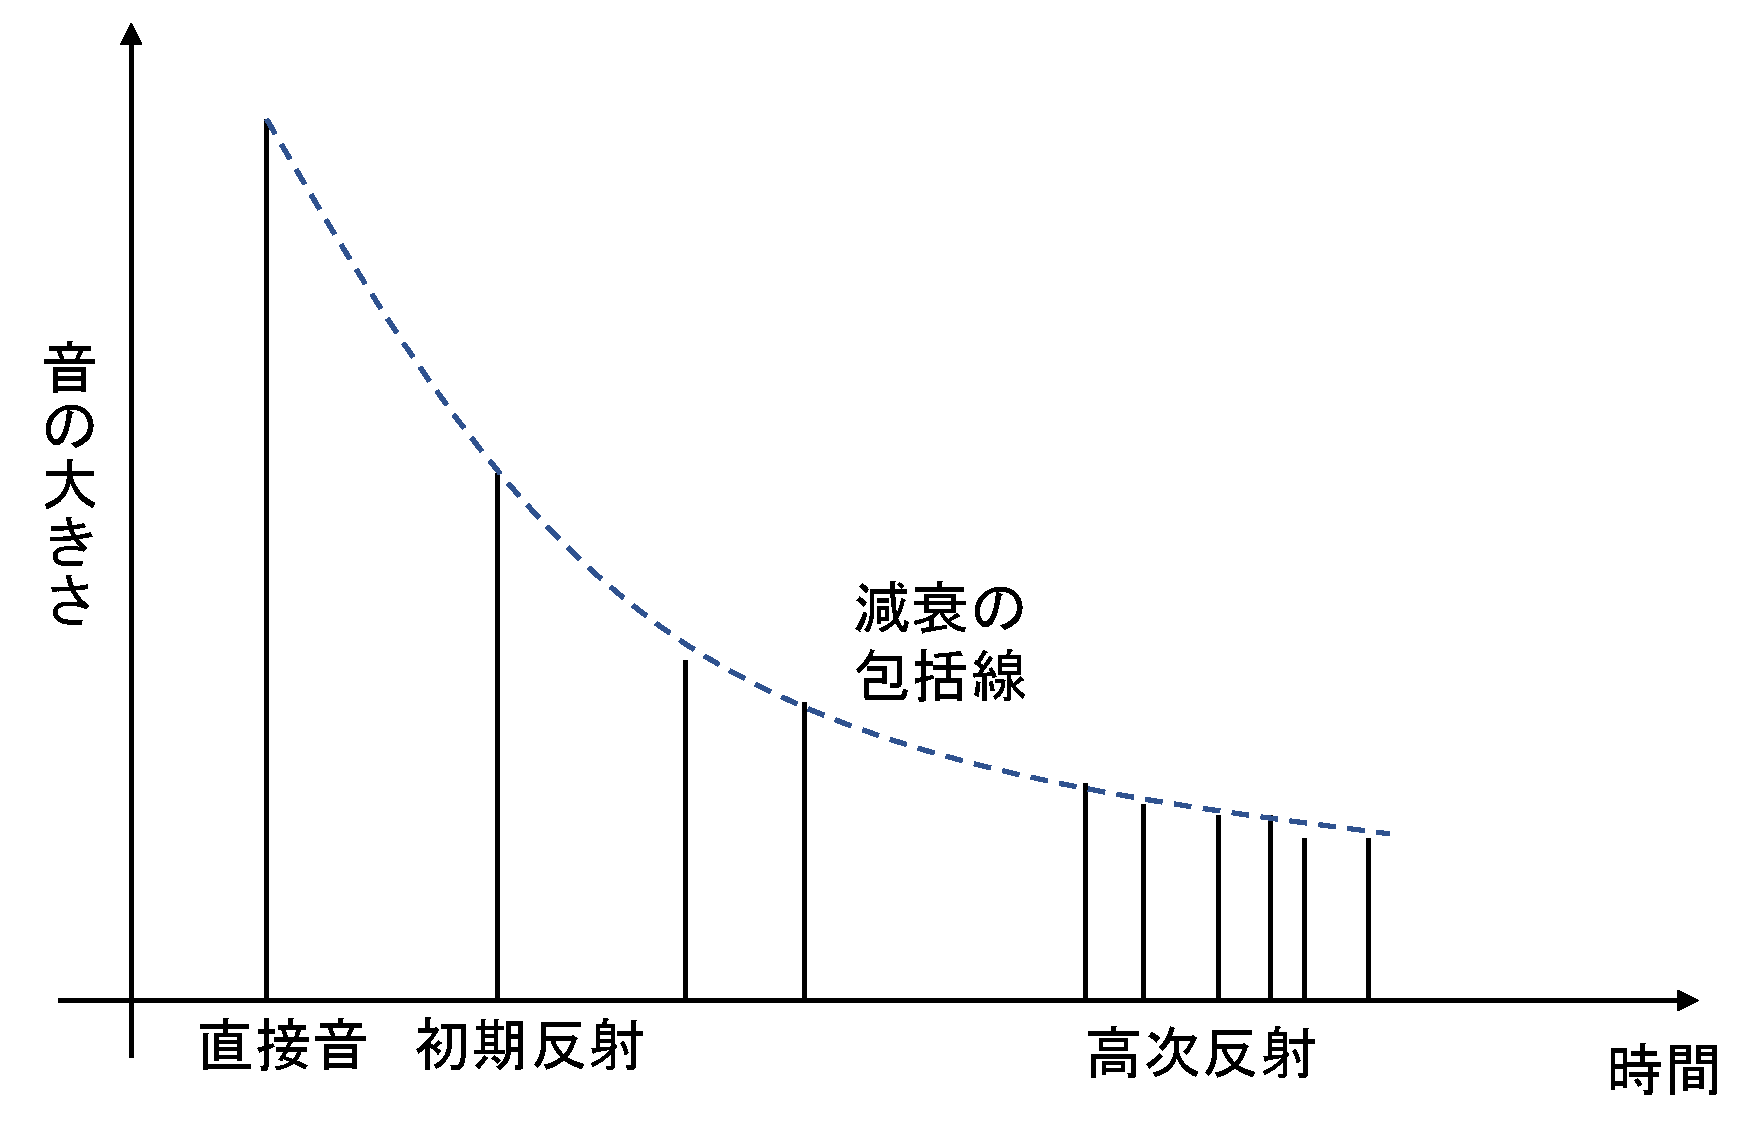
\includegraphics[clip,width=140mm,height=80mm]{ImpulseResponse.pdf}
\end{center}
 \caption{インパルス応答の例\cite{oka3}}
 \label{fig:impulse}
\end{figure}
\newpage
\subsection{伝達関数}
伝達関数とはシステムへの入力を出力に変換する関数のことをいう.伝達関数は,すべての初期値を0としたときの,制御系の出力と入力のラプラス変換(またはZ変換)の比で表される.すなわち,連続システムのとき,出力信号$y(t)$のラプラス変換を$Y(s)$,入力信号$x(t)$のラプラス変換を$X(s)$とすれば,伝達関数$G(s)$は
\begin{equation}
	\label{noref}
  G(s) =  \frac{Y(s)}{X(s)} = \frac{\mathcal{L}[y(t)]}{\mathcal{L}[x(t)]}
\end{equation}

と表される.
離散システムに対して,伝達関数はZ変換によって,
\begin{equation}
	\label{noref}
  H(z) =  \frac{Y(z)}{X(z)} = \frac{\mathcal{Z}[y(n)]}{\mathcal{Z}[x(n)]}
\end{equation}
と表される.
この伝達関数法では,時間領域の関数を,ラプラス変換(またはZ変換)によって複素平面に写像を取り,さらに周波数領域に変換することにより,系の特性や安定性を解析するのに用いる.ただし,対象となる系が1入力1出力(線形関数)に限られているため,複雑な系(多入力多出力,非線形)の解析には状態空間法を用いる.

インパルス応答をフーリエ変換して周波数領域で表現したものを伝達関数という.




\subsection{ノイズ}
ノイズとは,処理対象となる情報以外の不要な情報のことである.歴史的理由から雑音に代表されるため,しばしば工学分野の文章では音以外に関しても「雑音」と訳したり表現したりして,音以外の信号等におけるノイズの意味で扱っていることがある.マイク録音を行ったときに不用意な音まで録音されてしまうことがある.それらの不要な成分を総称してノイズと呼ぶ.ノイズは正確な音声信号処理を阻害する要因となるため除去するのが望ましいが,非常に不規則な値を取るため手がかりなしで適切に除去することは困難である.

不規則なノイズに対して,統計的な性質を知ることが重要であり,ホワイトノイズは代表的なモデルとして頻繁に使用される.
ホワイトノイズ例を図\ref{fig:whitenoize}に示す.

% 図5.4-1
\begin{figure}[h]
\begin{center}
 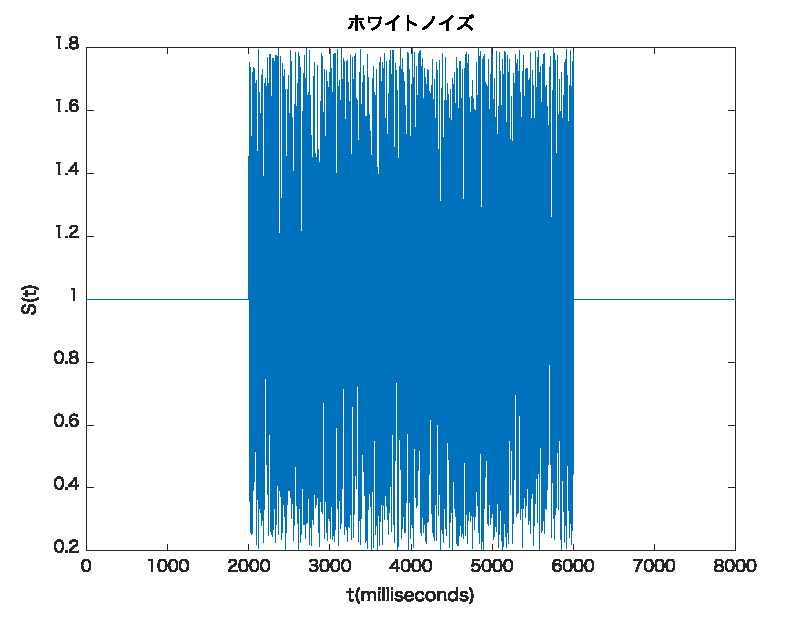
\includegraphics[clip,width=85mm,height=65mm]{whitenoize.pdf}
\end{center}
 \caption{ホワイトノイズ}
 \label{fig:whitenoize}
\end{figure}

\subsection{残響推定方法}
残響推定方法には二種類あり,ノイズ断続法とインパルス応答積分法の2つになる.

\subsubsection{ノイズ断続法}
この手法は,スピーカから試験音を放射し,試験音が部屋に充満したら,音を停止した後の音圧レベルを記録して残響時間を読み取る方法である.
\subsubsection{インパルス応答積分法}
この手法は,測定した音源点と受音点間のインパルス応答から求めた残響減衰曲線の傾きで残響時間を推定する方法である.
\newpage
\section{反射音除去の提案}
\subsection{パワースペクトルとクロススペクトル}
パワースペクトルとは信号のパワーを一定の周波数帯域に分割し,各帯域ごとのパワーを周波数の関数として表したものをいう.単位は振幅の2乗となる.また,パワースペクトルは波形の周波数成分をエネルギーとして表したものであり,その波形がどれほどのエネルギーを持っているかがわかる.\cite{oka6}

クロススペクトルとは2つの信号のスペクトルのある周波数どうしを掛け合わせたうえで平均化したもので,X軸は周波数,Y軸は$V^2$で表される.
クロススペクトルがある周波数において大きな値を示していた場合,その周波数において2信号の相関が大きいことがわかる.また,クロススペクトルは伝達関数,相互相関関数,コヒーレンス関数に使われる.\cite{oka6}
\subsection{クロススペクトル推定法}
自己相関関数,相互相関数ををフーリエ変換することで,それぞれのパワースペクトル密度関数,クロススペクトル密度が得られる.これを式で書くと,式\ref{powerspec},\ref{crossspec}のようになる.

\begin{equation}
\label{powerspec}
  S_x(f) = \int^{\infty}_{-\infty} R_x(\tau)e^{-j\omega \tau}{d\tau}
\end{equation}

\begin{equation}
\label{crossspec}
  S_{xy}(f) = \int^{\infty}_{-\infty} R_{xy}(\tau)e^{-j\omega \tau}{d\tau}
\end{equation}

更に時間領域の畳み込みの関係が周波数領域では席となる合成積則より
\begin{equation}
\label{crossspec}
  S_{xy}(f) = H(f)\cdot S_x(f)
\end{equation}

ここに$H(f)$はインパルス応答の周波数領域表現である.したがって,
\begin{equation}
\label{crossspec}
  S_{xy}(f) = \frac {S_{xy}(f)}{S_x(f)}
\end{equation}
を求め,これを逆フーリエ変換することでインパルス応答が求められることになる.ここで,パワースペクトル密度と信号のフーリエ変換の関係により,
\begin{equation}
\label{crossspec}
  S_{x}(f) = E[X^{*}(f)X(f)]
\end{equation}

\begin{equation}
\label{crossspec}
  S_{xy}(f) = E[X^{*}(f)Y(f)]
\end{equation}
となることになり,つまりは観測した信号$x(t)$,$y(t)$か,実際のはその離散時間表現$x(n)$,$y(n)$のフーリエ変換を求めて,上記の演算を行うことでインパルス応答の推定が行えることになる.フーリエ変換を用いることができる,ということは演算時間短縮に関する大きなメリットにもなる.
\subsection{先行研究による手法}
非常放送には反射音が建物などにより付加してしまい内容を聞き取りづらいといったことが問題点として挙げられている.その反射音を除去するために佐藤はクロススペクトル法を用いて反射音の除去に取り組んだ.

手法としては元波形の前におらかじめ信号音を付加させておく.それをもとに反射度合いを推定するため,インパルス応答を求める.反射音の付加された音声をインパルス応答で割ることで反射音が除去できる.

計算内容としては元波形を$S(t)$,反射音の含まれた音声を$R(t)$とすると,
はじめに両波形をフーリエ変換することにより周波数成分を求める.

\begin{equation}
  S(f) = \mathcal{F}[S(t)]
\end{equation}

\begin{equation}
  R(f) = \mathcal{F}[R(t)]
\end{equation}
 
元波形の周波数成分を二乗する(\ref{power})ことでパワースペクトル$P(f)$,元波形の周波数成分と反射音の含んだ波形の周波数成分の積(\ref{cross})によりクロススペクトル$C(f)$を求めることができる.
\begin{equation}
	\label{power}
  P(f) = [S(f)]^2
\end{equation}

\begin{equation}
	\label{cross}
  C(f) = [S(f)]・[R(f)]
\end{equation}

クロススペクトルをパワースペクトルで除算すること(\ref{transfer})により伝達関数$H(f)$を求めることができ,伝達関数を逆フーリエ変換すること(\ref{IR})によりインパルス応答$IR(t)$を求めることができる.
\begin{equation}
	\label{transfer}
  H(f) = \frac{C(f)}{P(f)}
\end{equation}

\begin{equation}
	\label{IR}
  IR(t) = \mathcal{F}^{-1}[H(f)]
\end{equation}

求めたインパルス応答を用いて,反射音の付加している音声の周波数成分をインパルス応答で除算すること(\ref{norefcomp})により反射音の除去された音声の周波数成分$N(f)$を求めることができる.またそれを逆フーリエ変換すること(\ref{noref})により反射音の除去された音声$N(t)$を取り出すことができる.

\begin{equation}
	\label{norefcomp}
  N(f) = \frac{R(f)}{IR(t)}
\end{equation}

\begin{equation}
	\label{noref}
  N(t) = \mathcal{F}^{-1}[N(f)]
\end{equation}

\begin{equation}
  N(t)\simeq S(t)
\end{equation}


\subsection{畳み込みと逆畳み込み}
畳み込みとはある関数$g$を平行移動させながら他の関数$f$に重ね足し合わせていく二項演算である.畳み込み積分,合成積,重畳積分,あるいは,英語にならいコンボリューションとも呼ばれる.画像処理や音響技術においてわざとノイズを付加させるときに使う事が多い.

逆畳み込みは,手順としては畳み込みの逆になる.画像処理においてブラインドデコンボリューションとして元画像がよくわからない状態からノイズ除去をしていく手段として使われることがある.近年では,ニューラルネットワークの分野で使われることが多い.
\subsection{ケプストラム法}
ケプストラムとはスペクトルの綴である「spectrum」の最初の4文字を逆にして考案された造語である.ケプストラムとは基本的に周波数特性のIDFTであるため,物理量の次元は時間である.ただし,通常のIDFTと区別するため,ケプストラムの次元は「ケフレンシー(quefrency)」と呼ばれている.これも周波数の綴である「frequency」をもじって考案された造語である\cite{oka4}.

ケプストラムの定義は以下のようになる.
\begin{eqnarray*}
 x_{c}(m) = \frac{1}{N}\sum^{N-1}_{k=0} log|X(k)|exp[\frac{j2\pi km}{N}]   
 \begin{array}{l}
 (0 \leq m \leq N-1)
 \end{array}
\end{eqnarray*}

\newpage

\subsection{提案手法}
本研究では,反射音が直接音に畳み込まれているものとして,反射音を付加した音声を元信号で逆畳み込みをすることで反射音を求められると考えた.また,反射音が付加されている音声から反射音を除去するために信号同士の計算が簡単になるケプストラム法を用いて反射音の除去された信号の抽出が可能である.

逆畳み込みによって求められた反射音D$(t)$,反射音が含まれた音声R$(t)$,放送内容のの音声S$(t)$
とすると図\ref{fig:cepstrum}のように表すことができる.


\begin{figure}[h]
\begin{center}
 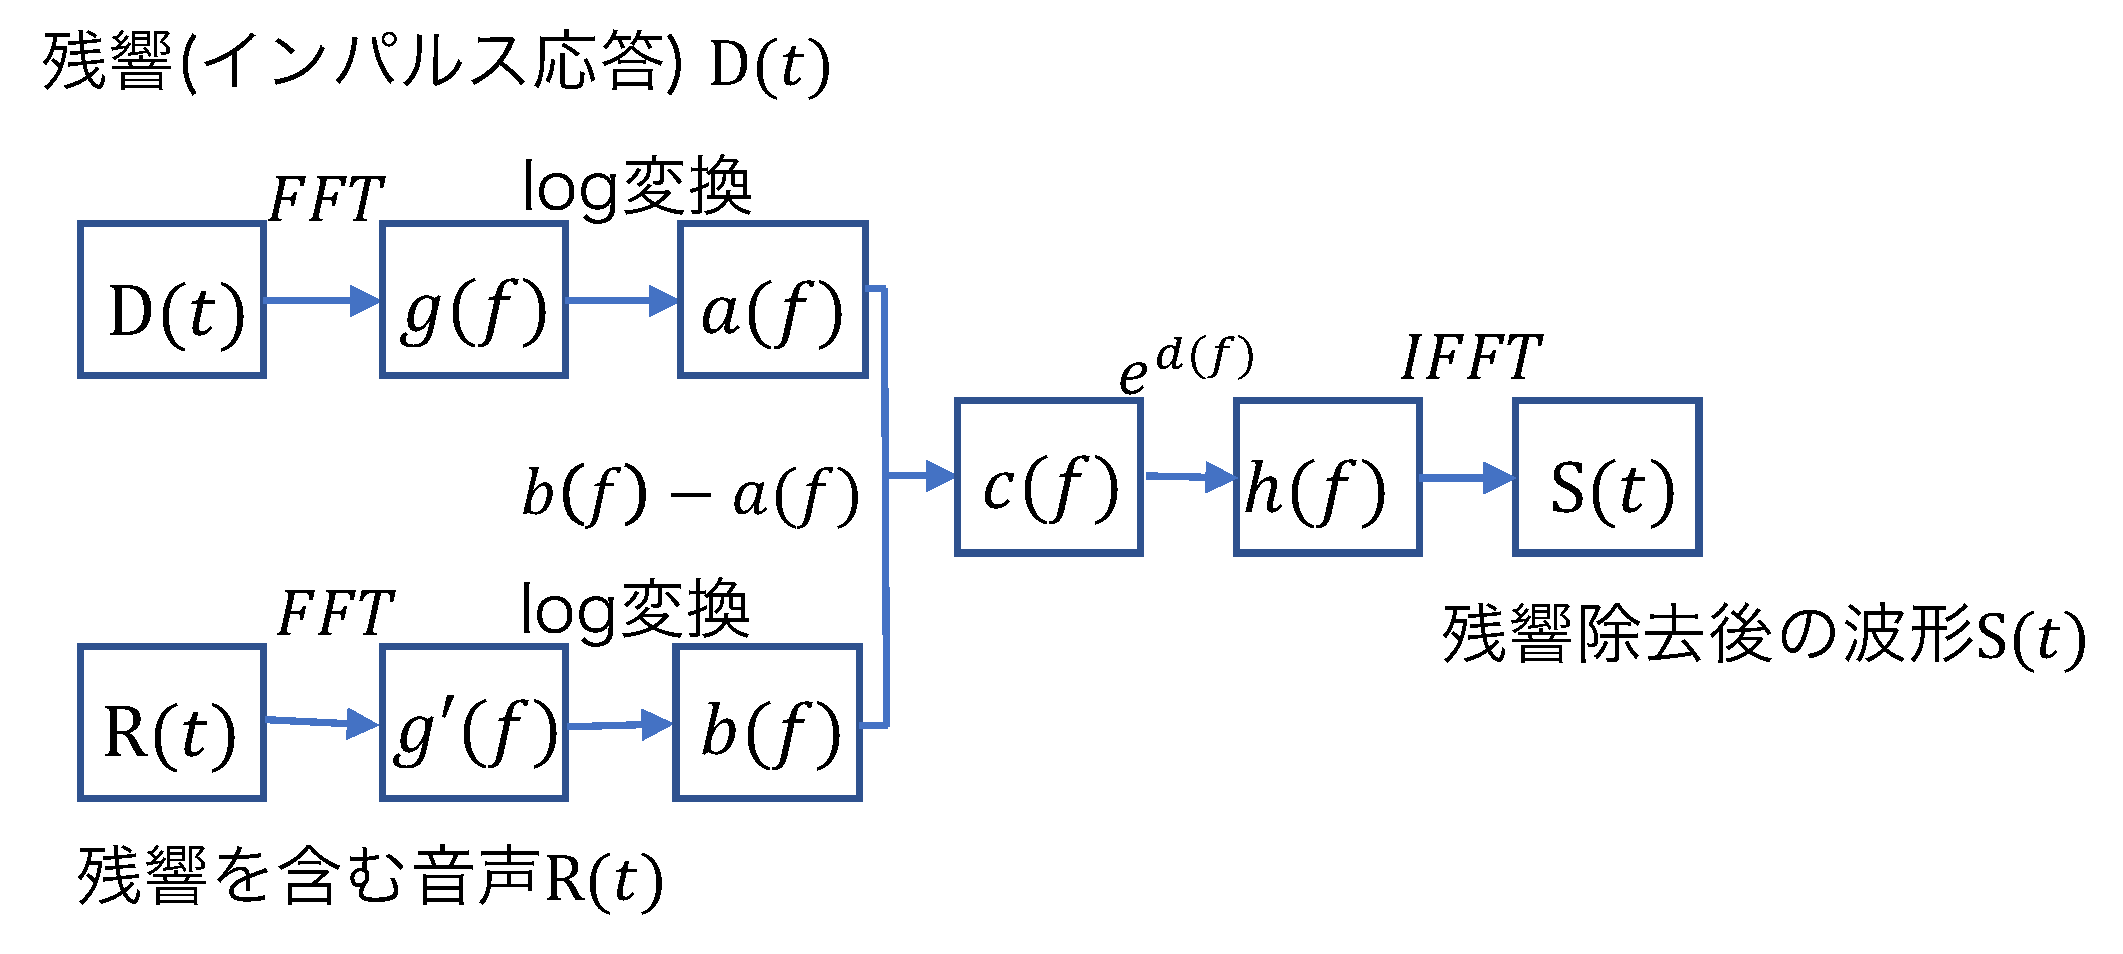
\includegraphics[clip,width=140mm,height=65mm]{riron.pdf}
\end{center}
 \caption{演算理論}
 \label{fig:cepstrum}
\end{figure}


\newpage
\section{実験と検証}
\subsection{調査目的}
今回の実験の調査目的は本研究で研究した残響除去を行った場合,正しく聞き取れることができるかどうかである.よって,複数人に対して聴覚実験を行った.本研究の聴覚実験では,残響音を付与した音声波形と,その波形から残響音除去の処理を施した音声の波形を用いた.地震発生時を想定した際の避難を促す文章や,津波警報が発令時に避難を促す文章など6秒から18秒の音声を計4編用意した.この4編に対して,残響を擬似的に付加させた音声とその残響を除去した音声,計8編を実験に用いた.被験者には残響音付きの音声2編と除去後の音声2編の計4編を無作為に聞いたもらった.聞きながら文章を書き出してもらい,正答率を式\ref{seitouritu}とした.
\begin{equation}
	\label{seitouritu}
  正答率 = \frac{聞き取れた文字数}{放送内容の文字数}
\end{equation}

放送内容を以下に示す.
\begin{itemize}
\item 緊急地震速報,強い揺れに警戒してください.\\
揺れが収まるまで安全を確保してください.
\item 津波警報が発令されました.\\
海岸付近の方は高台に避難してください.
\item こちらは防災センターです.\\
先程,火災感知器が作動しましたが,現場を確認した結果,誤報であることが確認できましたのでご安心ください.
\item 暴風警報が発令されました.\\
市内の皆様は,最寄りの避難所に避難してください.
\end{itemize}

\newpage
\subsection{調査方法}
今回,実施した残響除去が有用であるかどうかを検証するために複数人に対し,聴覚実験の協力をしたもらった.

今回使用した実行環境を表\ref{tab:use}に示す.

\begin{table}[htb]
\caption{実行環境}
  \begin{tabular}{|c|c|} \hline
    パソコン & iMac  \\ \hline
    OS & --  \\ \hline
    数値計算ソフトウェア & MATLAB\_R2019B  \\ \hline
    マルチメディアプレイヤー & --  \\ \hline
    使用ヘッドホン & audio-technica ATH-ES10  \\ \hline
    実験協力人数 & 6名  \\ \hline
    音声サンプルレート & 44,100Hz  \\ \hline
    ビット/サンプル & 16ビット/サンプル  \\ \hline
    チャンネル数 & モノラル  \\ \hline
    実験場所 & 津田沼校舎,7号館7階第12研究室\\ \hline
  \end{tabular}
  \label{tab:use}
\end{table}
\subsection{回答の集計と効果の検証}
今回の実験結果,文章の正答率を図\ref{fig:shitsumonshi},回答例を図\ref{fig:kinyurei}に示す.
\newpage
\begin{figure}[h]
\begin{center}
 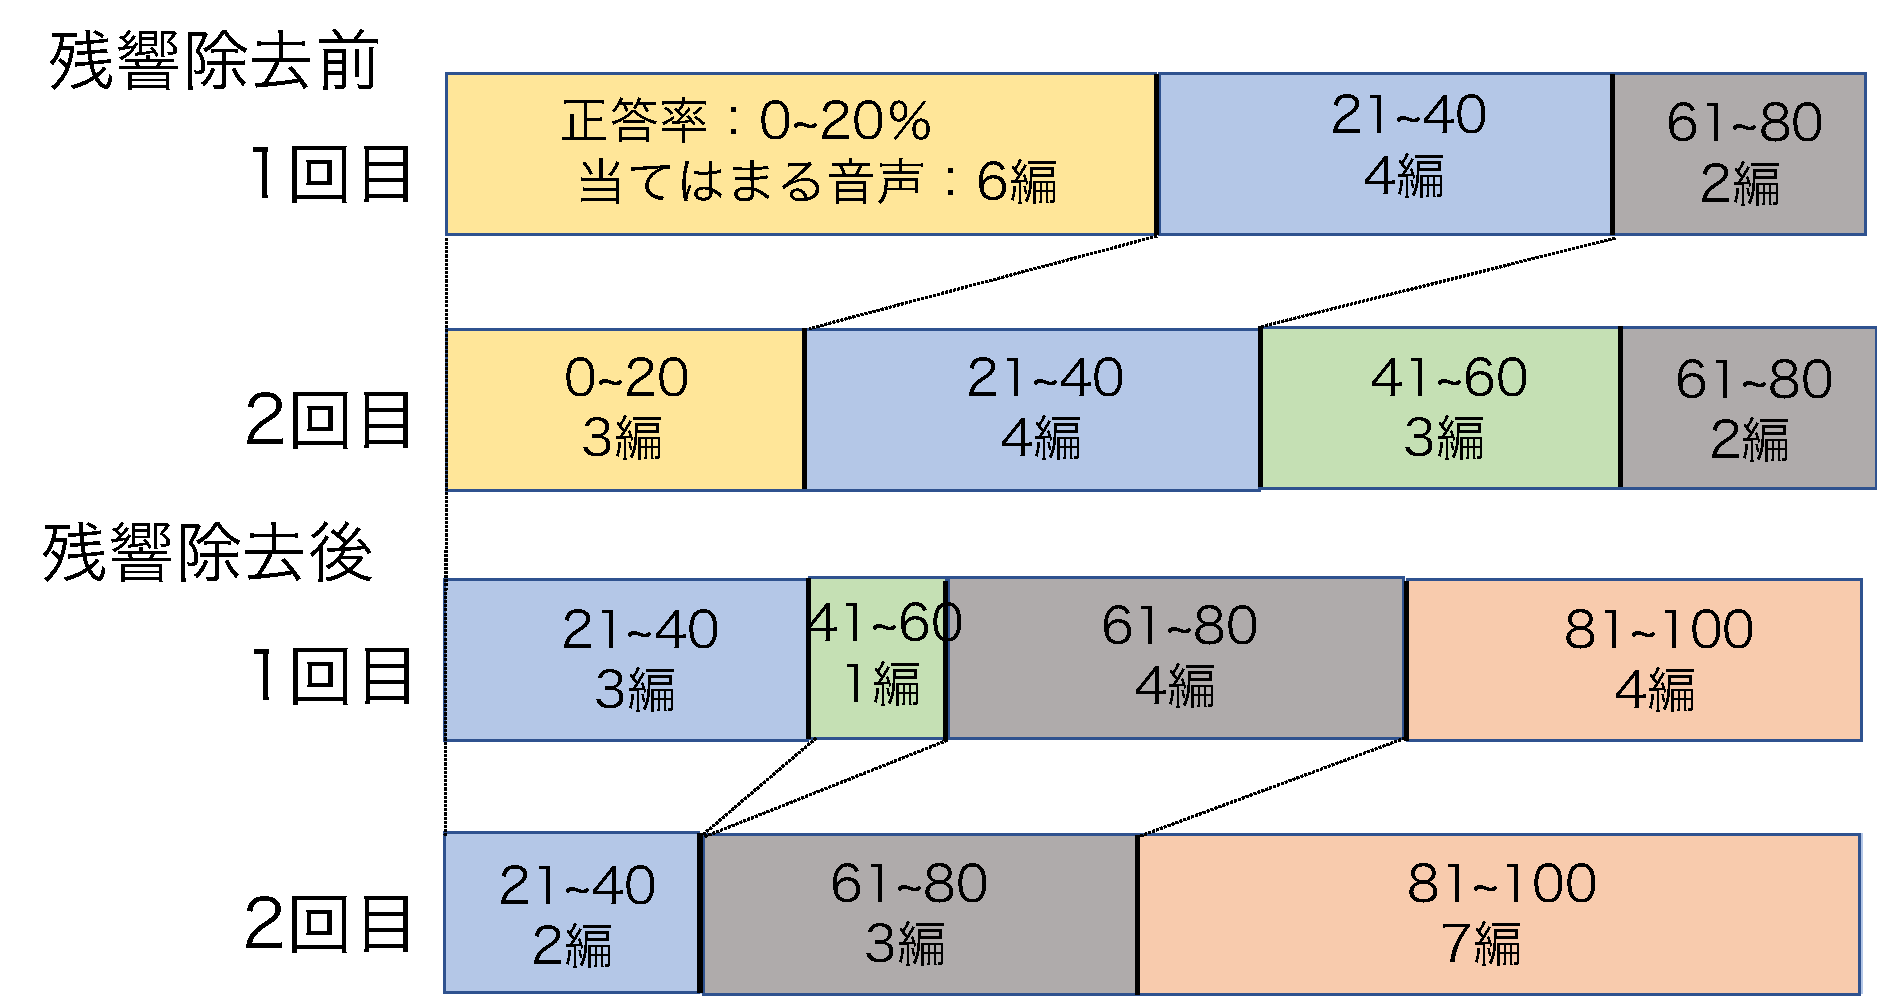
\includegraphics[clip,width=130mm,height=65mm]{shitsumonkekka.pdf}
\end{center}
 \caption{実験結果}
 \label{fig:shitsumonshi}
\end{figure}

\begin{figure}[h]
\begin{center}
 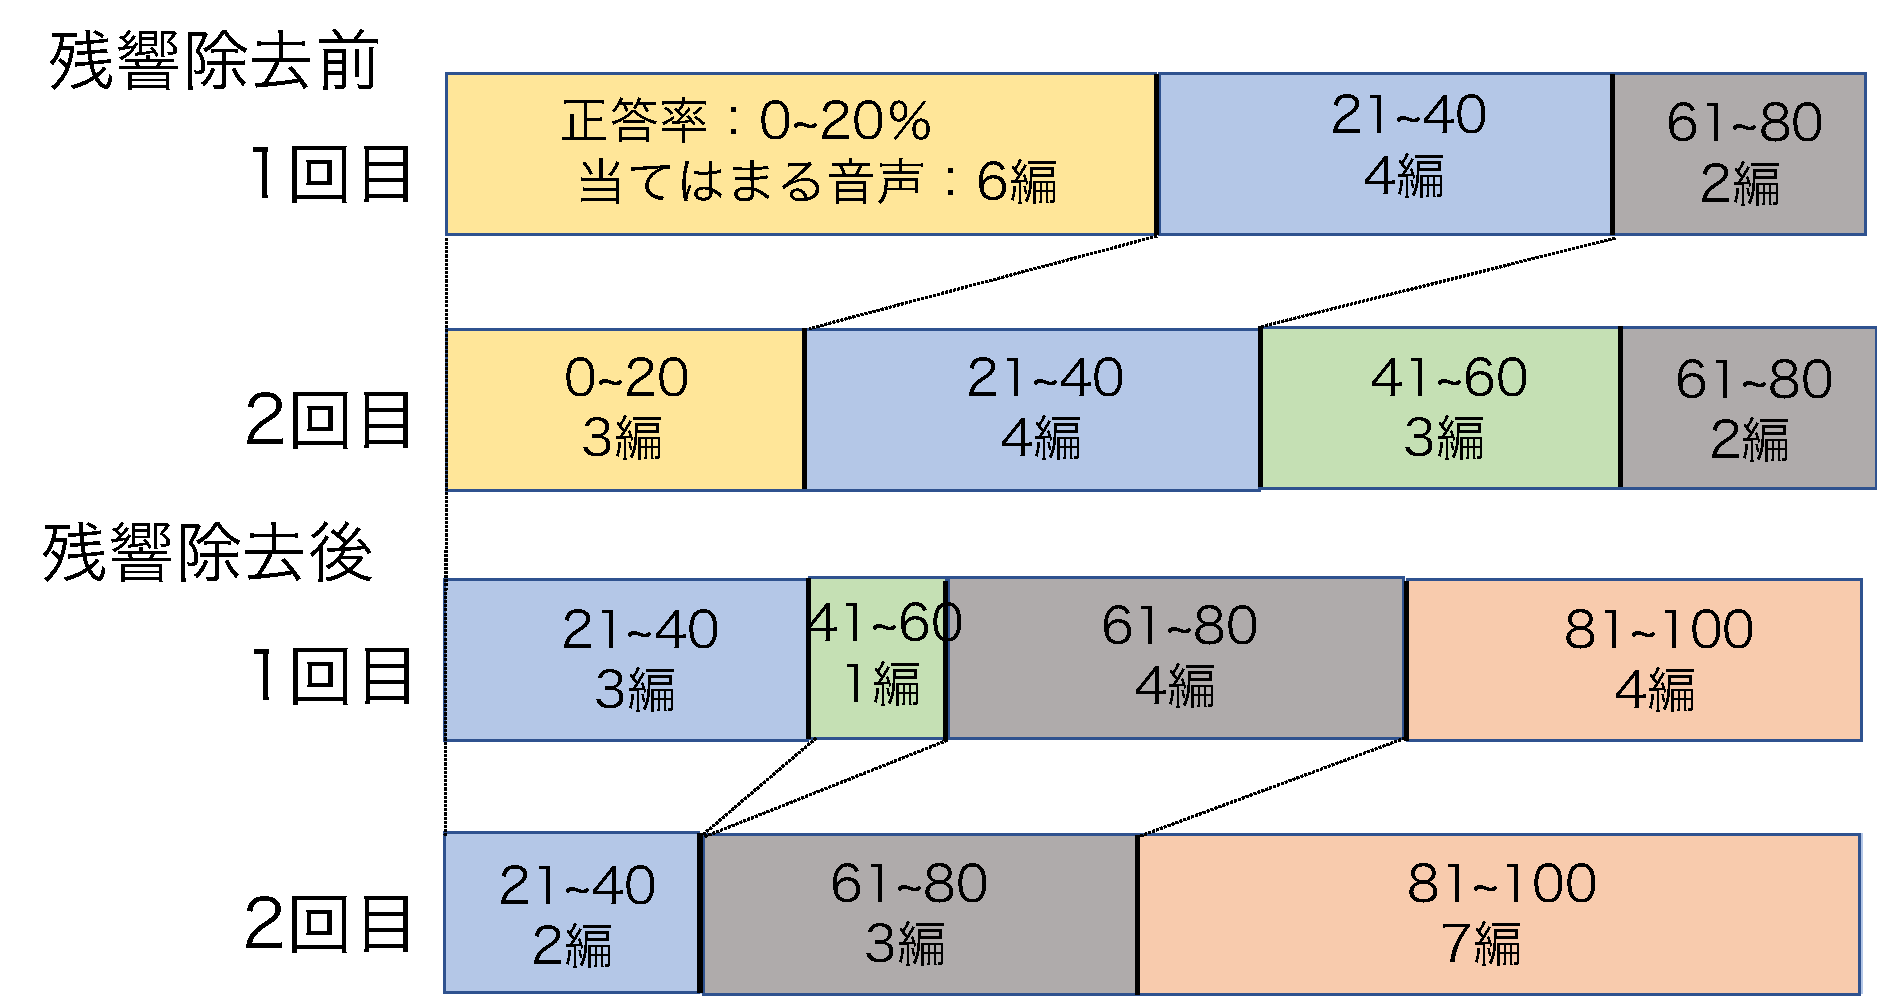
\includegraphics[clip,width=130mm,height=65mm]{shitsumonkekka.pdf}
\end{center}
 \caption{記入例}
 \label{fig:kinyurei}
\end{figure}
除去前の音声では1回目では6編(50\%)の音声の正答率が0	\textasciitilde20\%になっていることからも聞き取りづらいことがよく分かる.
また,2回聞いて61\%以上聞き取れているものが2編(20\%)だったのに対し,
除去後の音声では1回しか聞いていないにもかかわらず61\%以上聞き取れている音声が8編(70\%)あることからも聞き取りやすくなっていることがわかる.

加えて行った放送内容が理解できたかという問いに対しても残響を付加している音声より除去後の音声のほうが内容を理解して聞き取れていることがわかる.
\newpage

\subsection{考察}
逆畳込みとケプストラム法を組み合わせた音声による聴覚実験において,残響除去は成功し,放送内容を聞き取りやすくなったと考えられる.また,今回の実験では6名と比較的に少数による実験であったが,もっと多くの人数と多くの音声サンプルを用いれば,よりはっきりとした違いが現れるだろう.

しかし,今回の実験,検証において残響音を擬似的に畳み込んだものを使用している.実際の行政放送に対して使用できるかはこれから検証していく必要がある.

\newpage
\section{結言}

\newpage
\section*{謝辞}
\addcontentsline{toc}{section}{謝辞}
ここに研究の謝辞.主にご協力いただいた方など.

\newpage
\bibliographystyle{jplain}
\addcontentsline{toc}{section}{参考文献}
\begin{thebibliography}{99}

\bibitem{oka1}国土技術センター,``自然災害の多い国'',
http://www.jice.or.jp/knowledge/japan/commentary09
\bibitem{oka2}佐藤 由希子,``インパルス応答を用いた反射音除去のための一提案'', 千葉工業大学卒業論文, 2014
\bibitem{oka3}小泉 宣夫,``基礎音響・オーディオ学'',コロナ社 ,2005
\bibitem{oka4}青木 直史,``デジタル・サラウンド処理入門'',CQ出版,2006
\bibitem{oka5}日本音響学会編,``音響学入門ペディア'',コロナ社,2017
\bibitem{oka6}小野測器,``FFT解析に関する基礎用語集'',
\url{https://www.onosokki.co.jp/HP-WK/c_support/tech_term/cf_fft/cf3.htm}

\end{thebibliography}

\newpage
\section*{付録}
\addcontentsline{toc}{section}{付録}

\end{document}
